%!TEX root = JakubJedryszek-MasterThesis.tex

\cleardoublepage

\chapter{Verification}
\label{verification}

% meeting with Hatcliff: check for runtime exceptions, flow analysis based on derives, see photo/whiteboard

The strategy for Software Verification using SPARK tools is as follows. First, Examiner generates and discharge some Verification Conditions (VCs) and Dead Path Conjectures (DPCs). Next, SPARKSimp runs Simplifier to simplify and discharge some (or all) VCs, which were not discharged by Examiner. SPARKSimp runs also ZombieScope to analyze DPCs and ViCToR to discharge VCs (not discharged by Examiner nor Simplifier) with SMT Solver. To get summary of results, POGS report is generated. In case, when not all Verification Conditions are discharged, analysis continues with Bakar Kiasan. After fixes made with Kiasan help, Examiner and SPARKSimp tools are run again to confirm correctness. This approach is presented in the figure \ref{figure:sparkverificationstrategy}. Detailed overview of SPARK verification tools can be found in chapter 12 of SPARK book \cite{Barnes:Book}.

\begin{figure}[ht]%t=top, b=bottom, h=here
    \begin{center}
        
\includegraphics[width=1.0\textwidth]{figures/spark-verification.png}        
    \end{center}
    \caption{SPARK verification strategy}
    \label{figure:sparkverificationstrategy}
\end{figure}

\section{Verification of implemented prototype}
\label{verification:prototype}

During PCA pump prototype implementation, syntax was regularly checked with SPARK Examiner. Complete, manually implemented prototype, which can be found in appendix \ref{Appendix:pca_ravenscar}, was verified with strategy given at the beginning of this chapter (excluding Bakar Kiasan, which does not handle Ravenscar programs). Thus SPARK Examiner, SPARKSimp (Simplifier, ZombieScope and ViCToR) and POGS were used. Package \lstinline{Pca_Engine} was excluded from verification, using \lstinline{--# hide} annotation, because it contains Ada code, which is non-valid SPARK. The result of this analysis, in the form of POGS report summary, is presented in listing \ref{listing:pca_ravenscar:pogs}. Full report can be found in appendix \ref{Appendix:pca_ravenscar:pogs}.

POGS report shows that 30\% (90) of VCs were discharged by Examiner and 61\% (183) by Simplifier. There are 29 undischarged VCs. In addition to VCs, DPCs were generated and 32 dead paths were found. Some undischarged VCs and dead paths come from procedures responsible for maximum dose monitoring. As mentioned in chapter \ref{background:sparkverification:sireum}, Bakar Kiasan does not support Ravenscar profile. Thus, to be able to analyze monitoring dosed amount of drug, separate, sequential module was created. Verification process of this module is described in section \ref{verification:pcapump:monitoring}.

\singlespacing
\begin{lstlisting}[frame=single, gobble=0, caption={Summary of POGS report for PCA Pump prototype}, label={listing:pca_ravenscar:pogs}]
Summary:

The following subprograms have undischarged VCs (excluding those proved false):

   2  /Users/jj/aadl-medical/pca-pump-beagleboard/pca_ravenscar/pca_operation/get_time_between_activations.vcg
   1  /Users/jj/aadl-medical/pca-pump-beagleboard/pca_ravenscar/pca_operation/integer_array_store/get.vcg
   1  /Users/jj/aadl-medical/pca-pump-beagleboard/pca_ravenscar/pca_operation/integer_array_store/inc.vcg
   1  /Users/jj/aadl-medical/pca-pump-beagleboard/pca_ravenscar/pca_operation/integer_array_store/put.vcg
   2  /Users/jj/aadl-medical/pca-pump-beagleboard/pca_ravenscar/pca_operation/integer_array_store/sum.vcg
   1  /Users/jj/aadl-medical/pca-pump-beagleboard/pca_ravenscar/pca_operation/max_drug_per_hour_watcher.vcg
   1  /Users/jj/aadl-medical/pca-pump-beagleboard/pca_ravenscar/pca_operation/patientbolus.vcg
  20  /Users/jj/aadl-medical/pca-pump-beagleboard/pca_ravenscar/pca_operation/rate_controller.vcg

Proof strategies used by subprograms
-------------------------------------------------------------------------
Total subprograms with at least one VC proved by examiner:             15
Total subprograms with at least one VC proved by simplifier:           20
Total subprograms with at least one VC proved by contradiction:         0
Total subprograms with at least one VC proved with user proof rule:     0
Total subprograms with at least one VC proved by Victor:                0
Total subprograms with at least one VC proved by Riposte:               0
Total subprograms with at least one VC proved using checker:            0
Total subprograms with at least one VC discharged by review:            0

Maximum extent of strategies used for fully proved subprograms:
-------------------------------------------------------------------------
Total subprograms with proof completed by examiner:                     0
Total subprograms with proof completed by simplifier:                  14
Total subprograms with proof completed with user defined rules:         0
Total subprograms with proof completed by Victor:                       0
Total subprograms with proof completed by Riposte:                      0
Total subprograms with proof completed by checker:                      0
Total subprograms with VCs discharged by review:                        0

Overall subprogram summary:
-------------------------------------------------------------------------
Total subprograms fully proved:                                        14
Total subprograms with at least one undischarged VC:                    8  <<<
Total subprograms with at least one false VC:                           0
                                                                    -----
Total subprograms for which VCs have been generated:                   22


ZombieScope Summary:
-------------------------------------------------------------------------
Total subprograms for which DPCs have been generated:                  22
Total number subprograms with dead paths found:                         3
Total number of dead paths found:                                      32


VC summary:
-------------------------------------------------------------------------
Note: (User) denotes where the Simplifier has proved VCs using one or
      more user-defined proof rules.

Total VCs by type:
------------------
                    Total   Examiner Simplifier    Undisc.
Assert/Post            93         80         12          1
Precondition           12          0         12          0
Check stmnt.            0          0          0          0
Runtime check         187          0        159         28
Refinem. VCs           10         10          0          0
Inherit. VCs            0          0          0          0
==========================================================
Totals:               302         90        183         29 <<<
%Totals:                         30%        61%        10%

===================== End of Semantic Analysis Summary ========================
\end{lstlisting}
\doublespacing



\section{Monitoring dosed amount}
\label{verification:pcapump:monitoring}

This section is case study of verification of module responsible for tracking dosed amount of drug. The module was created with sequential profile, based on implemented PCA prototype presented in appendix \ref{Appendix:pca_ravenscar}. Isolated module is presented in listing \ref{listing:pcapump_dosemonitor}.

\singlespacing
\begin{lstlisting}[language=ada, frame=single, gobble=0, caption={Dose monitor module specification}, label={listing:pcapump_dosemonitor}]
package Pca_Pump
--# own Dosed;
--#     Dose_Volume;
--# initializes Dosed,
--#             Dose_Volume;
is
    subtype Integer_Array_Index is Integer range 1 .. 60*60;
    type Integer_Array is array (Integer_Array_Index) of Integer;

    procedure Increase_Dosed;
    --# global in out Dosed;
    --#        in Dose_Volume;
    --# derives Dosed from Dosed, Dose_Volume;

    function Read_Dosed return Integer;
    --# global in Dosed;

    procedure Move_Dosed;
    --# global in out Dosed;
    --# derives Dosed from Dosed;

end Pca_Pump;

package body Pca_Pump
is
    Dosed : Integer_Array := Integer_Array'(others => 0);
    Dose_Volume : Integer := 1;

    procedure Increase_Dosed
    is
    begin
        Dosed(Integer_Array_Index'Last) := Dosed(Integer_Array_Index'Last) + Dose_Volume;
    end Increase_Dosed;

    function Read_Dosed return Integer
    is
        Result : Integer := 0;
    begin
        for I in Integer_Array_Index loop
            --# assert I > 1 -> Result >= Dosed(I-1);
            Result := Result + Dosed(I);
        end loop;
        return Result;
    end Read_Dosed;

    procedure Move_Dosed
    is
    begin
        for I in Integer_Array_Index range 1 .. Integer_Array_Index'Last-1 loop
            --# assert I > 1 -> Dosed(I-1) = Dosed(I);
            Dosed(I) := Dosed(I+1);
        end loop;
        Dosed(Integer_Array_Index'Last) := 0;
    end Move_Dosed;

end Pca_Pump;
\end{lstlisting}
\doublespacing

Verification strategy is the same like described at the beginning of the chapter and depicted in the figure \ref{figure:sparkverificationstrategy}. First, program is verified with Examiner, SPARKSimp (Simplifier, ZombieScope and Victor). Verification report is generated by POGS. In case of any issues, verification is continued with Bakar Kiasan, which gives more user friendly experience that POGS report and generated VC files. 

First verification report generated by POGS is presented in listing \ref{listing:pcapump_dosemonitor_pogs}. It indicates presence of three undischarged (not proved) VCs.

\singlespacing
\begin{lstlisting}[frame=single, gobble=0, caption={POGS report}, label={listing:pcapump_dosemonitor_pogs}]
-------------------------------------------------------------------------------
                          Semantic Analysis Summary                            
                                POGS GPL 2012                                  
            Copyright (C) 2012 Altran Praxis Limited, Bath, U.K.               
-------------------------------------------------------------------------------

Summary of:

Verification Condition files (.vcg)
Simplified Verification Condition files (.siv)
Victor result files (.vct)
Riposte result files (.rsm)
Proof Logs (.plg)
Dead Path Conjecture files (.dpc)
Summary Dead Path files (.sdp)

"status" column keys:
    1st character:
        '-' - No VC
        'S' - No SIV
        'U' - Undischarged
        'E' - Proved by Examiner
        'I' - Proved by Simplifier by Inference
        'X' - Proved by Simplifier by Contradiction
        'P' - Proved by Simplifier using User Defined Proof Rules
        'V' - Proved by Victor
        'O' - Proved by Riposte
        'C' - Proved by Checker
        'R' - Proved by Review
        'F' - VC is False
    2nd character:
        '-' - No DPC
        'S' - No SDP
        'U' - Unchecked
        'D' - Dead path
        'L' - Live path

in the directory:
/Volumes/External/VMS/shared/aadl-medical/pca-pump-beagleboard/Pca_Verification

Summary produced: 01-JUL-2014 14:43:18.04

File /Volumes/External/VMS/shared/aadl-medical/pca-pump-beagleboard/Pca_Verification/pca_pump/increase_dosed.vcg
procedure Pca_Pump.Increase_Dosed

VCs generated 01-JUL-2014 14:42:26

VCs simplified 01-JUL-2014 14:43:04

File /Volumes/External/VMS/shared/aadl-medical/pca-pump-beagleboard/Pca_Verification/pca_pump/increase_dosed.dpc
DPCs generated 01-JUL-2014 14:42:26

DPC ZombieScoped 01-JUL-2014  14:43:0

VCs for procedure_increase_dosed :
 -----------------------------------------------------------------------------
| #   | From  | To                  | Proved By          | Dead Path | Status |
|-----------------------------------------------------------------------------
| 1   | start | rtc check @ 9       | Undischarged       | Unchecked |   UU   |
| 2   | start |    assert @ finish  | Examiner           | Live      |   EL   |
 -----------------------------------------------------------------------------


File /Volumes/External/VMS/shared/aadl-medical/pca-pump-beagleboard/Pca_Verification/pca_pump/move_dosed.vcg
procedure Pca_Pump.Move_Dosed

VCs generated 01-JUL-2014 14:42:26

VCs simplified 01-JUL-2014 14:43:04

File /Volumes/External/VMS/shared/aadl-medical/pca-pump-beagleboard/Pca_Verification/pca_pump/move_dosed.dpc
DPCs generated 01-JUL-2014 14:42:26

DPC ZombieScoped 01-JUL-2014  14:43:0

VCs for procedure_move_dosed :
 -----------------------------------------------------------------------------
| #   | From  | To                  | Proved By          | Dead Path | Status |
|-----------------------------------------------------------------------------
| 1   | start | rtc check @ 26      | Inference          | Unchecked |   IU   |
| 2   | start | rtc check @ 26      | Inference          | Unchecked |   IU   |
| 3   | start |    assert @ 27      | Inference          | Live      |   IL   |
| 4   | 27    |    assert @ 27      | Inference          | Live      |   IL   |
| 5   | 27    | rtc check @ 28      | Inference          | Unchecked |   IU   |
| 6   | start | rtc check @ 30      | Inference          | Unchecked |   IU   |
| 7   | 27    | rtc check @ 30      | Inference          | Unchecked |   IU   |
| 8   | start |    assert @ finish  | Examiner           | Dead      |   ED   |
| 9   | 27    |    assert @ finish  | Examiner           | Live      |   EL   |
 -----------------------------------------------------------------------------


File /Volumes/External/VMS/shared/aadl-medical/pca-pump-beagleboard/Pca_Verification/pca_pump/read_dosed.vcg
function Pca_Pump.Read_Dosed

VCs generated 01-JUL-2014 14:42:26

VCs simplified 01-JUL-2014 14:43:05

File /Volumes/External/VMS/shared/aadl-medical/pca-pump-beagleboard/Pca_Verification/pca_pump/read_dosed.dpc
DPCs generated 01-JUL-2014 14:42:26

DPC ZombieScoped 01-JUL-2014  14:43:0

VCs for function_read_dosed :
 -----------------------------------------------------------------------------
| #   | From  | To                  | Proved By          | Dead Path | Status |
|-----------------------------------------------------------------------------
| 1   | start |    assert @ 17      | Inference          | Live      |   IL   |
| 2   | 17    |    assert @ 17      | Undischarged       | Live      |   UL   |
| 3   | 17    | rtc check @ 18      | Undischarged       | Unchecked |   UU   |
| 4   | 17    |    assert @ finish  | Inference          | Live      |   IL   |
 -----------------------------------------------------------------------------


===============================================================================
Summary:

The following subprograms have undischarged VCs (excluding those proved false):

   1  /Volumes/External/VMS/shared/aadl-medical/pca-pump-beagleboard/Pca_Verification/pca_pump/increase_dosed.vcg
   2  /Volumes/External/VMS/shared/aadl-medical/pca-pump-beagleboard/Pca_Verification/pca_pump/read_dosed.vcg

Proof strategies used by subprograms
-------------------------------------------------------------------------
Total subprograms with at least one VC proved by examiner:              2
Total subprograms with at least one VC proved by simplifier:            2
Total subprograms with at least one VC proved by contradiction:         0
Total subprograms with at least one VC proved with user proof rule:     0
Total subprograms with at least one VC proved by Victor:                0
Total subprograms with at least one VC proved by Riposte:               0
Total subprograms with at least one VC proved using checker:            0
Total subprograms with at least one VC discharged by review:            0

Maximum extent of strategies used for fully proved subprograms:
-------------------------------------------------------------------------
Total subprograms with proof completed by examiner:                     0
Total subprograms with proof completed by simplifier:                   1
Total subprograms with proof completed with user defined rules:         0
Total subprograms with proof completed by Victor:                       0
Total subprograms with proof completed by Riposte:                      0
Total subprograms with proof completed by checker:                      0
Total subprograms with VCs discharged by review:                        0

Overall subprogram summary:
-------------------------------------------------------------------------
Total subprograms fully proved:                                         1
Total subprograms with at least one undischarged VC:                    2  <<<
Total subprograms with at least one false VC:                           0
                                                                    -----
Total subprograms for which VCs have been generated:                    3


ZombieScope Summary:
-------------------------------------------------------------------------
Total subprograms for which DPCs have been generated:                   3
Total number subprograms with dead paths found:                         1
Total number of dead paths found:                                       1


VC summary:
-------------------------------------------------------------------------
Note: (User) denotes where the Simplifier has proved VCs using one or
      more user-defined proof rules.

Total VCs by type:
------------------
                    Total   Examiner Simplifier    Undisc.
Assert/Post             8          3          4          1
Precondition            0          0          0          0
Check stmnt.            0          0          0          0
Runtime check           7          0          5          2
Refinem. VCs            0          0          0          0
Inherit. VCs            0          0          0          0
==========================================================
Totals:                15          3          9          3 <<<
%Totals:                         20%        60%        20%

===================== End of Semantic Analysis Summary ========================
\end{lstlisting}
\doublespacing

Next, according to verification strategy, Bakar Kiasan was run. Kiasan report is presented in the figure \ref{figure:sparkverification:kiasanreport1}.

\begin{figure}[ht]%t=top, b=bottom, h=here
    \begin{center}
        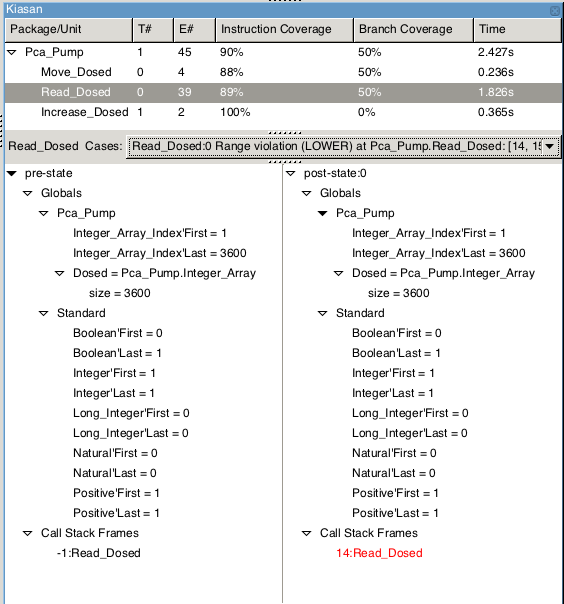
\includegraphics[width=0.8\textwidth]{figures/pca-pump-verification-step1.png}        
    \end{center}    
    \caption{Bakar Kiasan verification report}
    \label{figure:sparkverification:kiasanreport1}
\end{figure}

First issue we can notice is problem with data types' ranges. To solve it (in SPARK 2005) configuration file \lstinline{Standard.ads} (presented in listing \ref{figure:sparkverification:config}) was created. Kiasan verification report created after that is presented in the figure \ref{figure:sparkverification:kiasanreport2}. Number of errors is reduced, but there is still problem with range violation.

\singlespacing
\begin{lstlisting}[frame=single, gobble=0, caption={Configuration file for Bakar Kiasan}, label={figure:sparkverification:config}]
package Standard is

    type Integer is range -2**31 .. 2**31-1;

end Standard;
\end{lstlisting}
\doublespacing

\begin{figure}[ht]%t=top, b=bottom, h=here
    \begin{center}
        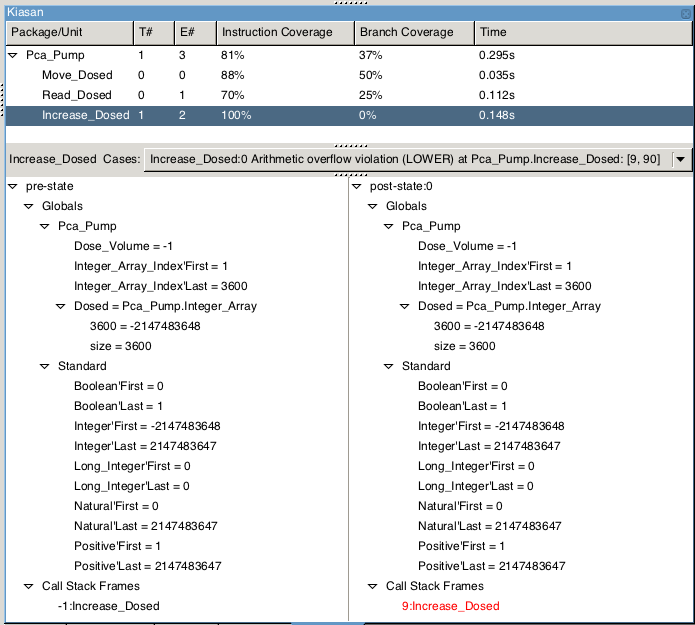
\includegraphics[width=0.8\textwidth]{figures/pca-pump-verification-step2.png}        
    \end{center}
    \caption{Bakar Kiasan verification report, second run}
    \label{figure:sparkverification:kiasanreport2}
\end{figure}

From functional perspective, negative values are not needed it this case, thus new type \lstinline{Drug_Volume} type was created. \lstinline{Integer_Array} type was renamed to \lstinline{Doses_Array} and its type was changed to \lstinline{Drug_Volume}. Result of Kiasan analysis after this change is presented in the figure \ref{figure:sparkverification:kiasanreport3}.

\begin{figure}[ht]%t=top, b=bottom, h=here
    \begin{center}
        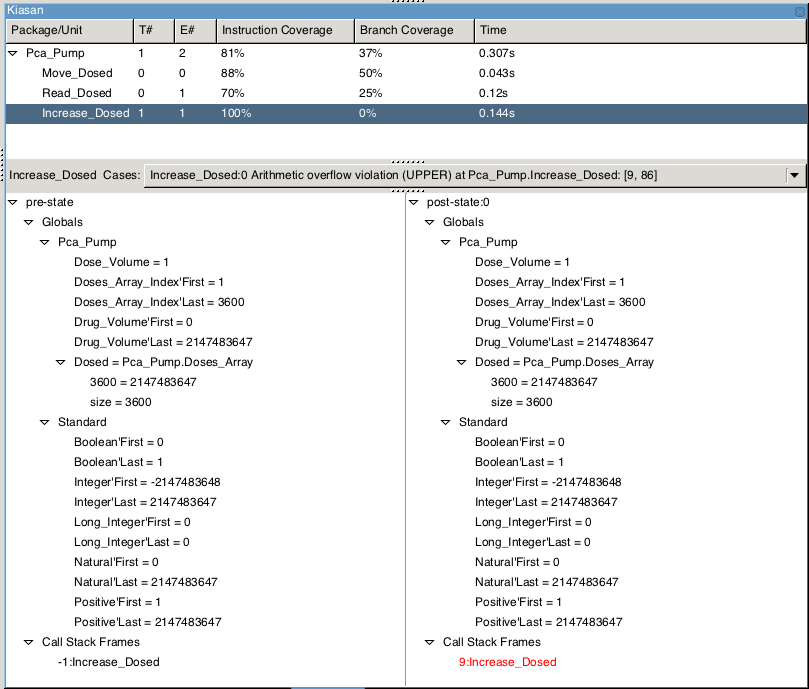
\includegraphics[width=0.8\textwidth]{figures/pca-pump-verification-step3.png}        
    \end{center}
    \caption{Bakar Kiasan verification report, third run}
    \label{figure:sparkverification:kiasanreport3}
\end{figure}

After this change, only upper overflow in \lstinline{Increase_Dosed} procedure error was left. Fix, for this is introduction of precondition for \lstinline{Increase_Dosed}: \lstinline{--# pre Read_Dosed(Dosed) <= Drug_Volume'Last - Dose_Volume;}. It caused semantic error (detected by Examiner): \lstinline{The identifier Read_Dosed is either undeclared or not visible at this point}. The reason of that is definition of \lstinline{Increase_Dosed} procedure before \lstinline{Read_Dosed} procedure. To fix, this \lstinline{Read_Dosed} procedure was moved before \lstinline{Increase_Dosed}. However, after that Examiner returned different error: \lstinline{Binary operator is not declared for types Drug_Volume and Dose_Volume__type}. To make operator visible, \lstinline{Dose_Volume} type has to be declared in \lstinline{--# own} annotation: \lstinline{--# Dose_Volume : Drug_Volume;}. After these fixes Kiasan analysis has be run again. Result is depicted in the figure \ref{figure:sparkverification:kiasanreport4}.

\begin{figure}[ht]%t=top, b=bottom, h=here
    \begin{center}
        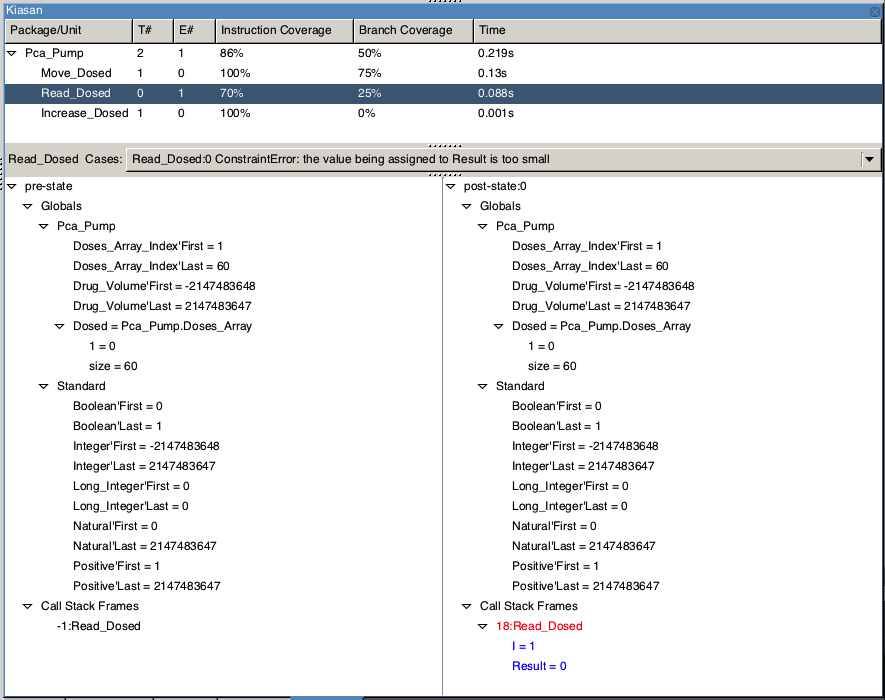
\includegraphics[width=0.8\textwidth]{figures/pca-pump-verification-step4.png}
    \end{center}
    \caption{Bakar Kiasan verification report, forth run}
    \label{figure:sparkverification:kiasanreport4}
\end{figure}

There were no error cases in \lstinline{Move_Dosed} and \lstinline{Increase_Dosed} procedures. Error case in \lstinline{Read_Dosed} is shown in figure \ref{figure:sparkverification:kiasanreport4}. It is \lstinline{ConstraintError: the value being assigned to Result is too small}. This error is not very imformative. After investigation and talk with Kiasan Developer, it was determined that there is a bug in Kiasan v1 (for SPARK 2005). More precisely: in checking overflows. For the purpose of verification \lstinline{Drug_Volume} type range was changed to $0 - (2^{15} - 1)$. It will give range up to around 1000000. Which is sufficient even if calculations are made in micro liters (as it is in case of PCA pump prototype implementation). 1000000 micro liters is 1000 ml, which is 1 liter. This is extreme amount of drug in case of PCA pump, according to Requirement Document \cite{OpenSourcePCAPump:Paper}. The bug with type ranges is fixed in Kiasan v2 (for SPARK 2014).

Another problem was the size of \lstinline{Dosed} array (3600 elements). Kiasan allows to set array bound and loop bound. Both had to be increased (from default 10). Another thing was computational complexity. For 3600 elements, state space grows exponentially and it takes a lot of time to analyze it. Thus, for verification purposes, array size was changed to 60 elements. Along with change to array bounds and loop bounds, also to 60.

After rerun Kiasan, there is valid test case for \lstinline{Read_Dose}, but there are also 59 Exception cases: \lstinline{Range violation (UPPER)}, which means possible overflow. One way of fix it, was to add \lstinline{--# assume} annotation to loop in function body, but Kiasan v1 does not support it. Another way was to add precondition, which assure, that sum of elements is lower than \lstinline{Drug_Volume'Last}. SPARK does not provide simple library for summing array (like Contracts language for Java provide). Thus, this function had to be implemented. Its implementation is the same like \lstinline{Read_Dosed}. It sum all elements of array. \lstinline{Sum} function specification and body is presented in listing \ref{listing:sum_function}.

\singlespacing
\begin{lstlisting}[language=ada, frame=single, gobble=0, caption={Sum function for summing all elements of array}, label={listing:sum_function}]
function Sum(Arr : Doses_Array) return Drug_Volume;

function Sum(Arr : Doses_Array) return Drug_Volume
is
    Result : Drug_Volume := 0;
begin
    for I in Doses_Array_Index loop
        --# assert true;
        Result := Result + Arr(I);
    end loop;
    return Result;
end Sum;
\end{lstlisting}
\doublespacing

After rerunning Kiasan, only valid test case were found, which is depicted in the figure \ref{figure:sparkverification:kiasanreport5}.

\begin{figure}[ht]%t=top, b=bottom, h=here
    \begin{center}
        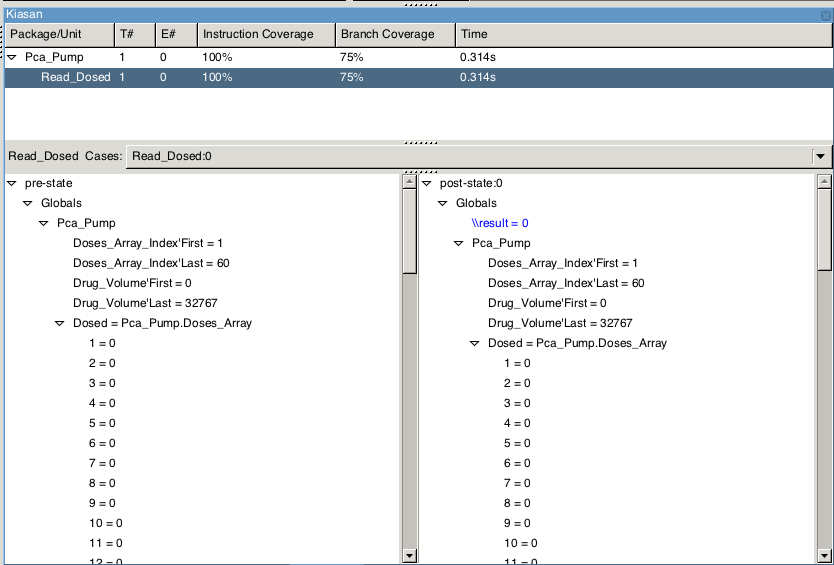
\includegraphics[width=0.8\textwidth]{figures/pca-pump-verification-step5.png}        
    \end{center}
    \caption{Bakar Kiasan verification report, fifth run}
    \label{figure:sparkverification:kiasanreport5}
\end{figure}

The last thing which was improved by code contracts is checking if \lstinline{Move_Dosed} procedure works as expected. In that purpose three postconditions were added (listing \ref{listing:postconditions_added_to_move_dosed}). First checks if the last element is equal to 0. Second and third checks two possible scenarios: 
\begin{itemize}
    \item before running procedure, the first element is equal to 0: amount of dosed drug in last hour will not change after Dosed procedure execution
    \item the first element is greater than 0: after Dosed procedure execution, the amount of drug dosed in last hour will decrease, because first element value will no longer be in last hour range
\end{itemize}

\singlespacing
\begin{lstlisting}[language=ada, frame=single, gobble=0, caption={Postconditions added to Move\_Dosed procedure}, label={listing:postconditions_added_to_move_dosed}]
--# post Dosed(Doses_Array_Index'Last) = 0 
--#      and (Dosed~(Doses_Array_Index'First)=0 -> Read_Dosed(Dosed~) = Read_Dosed(Dosed))
--#      and (Dosed~(Doses_Array_Index'First)>0 -> Read_Dosed(Dosed~) > Read_Dosed(Dosed));
\end{lstlisting}
\doublespacing

After adding these postconditions Kiasan generates 2 test cases to check both mentioned scenarios. There is no error cases, which means that procedure works as expected. 

Better way to validate such requirements is Unit testing. In section \ref{verification:aunit}, there is overview of unit tests created to test behavior described above.

To validate changes made, while working with Kiasan, SPARK Examiner and SPARKSimp were rerun again. POGS report is presented in listing \ref{listing:pcapump_dosemonitor_pogs3}.

\singlespacing
\begin{lstlisting}[frame=single, gobble=0, caption={Third POGS report}, label={listing:pcapump_dosemonitor_pogs3}]
VCs for procedure_increase_dosed :
 -----------------------------------------------------------------------------
| #   | From  | To                  | Proved By          | Dead Path | Status |
|-----------------------------------------------------------------------------
| 1   | start | rtc check @ 20      | Undischarged       | Unchecked |   UU   |
| 2   | start |    assert @ finish  | Examiner           | Live      |   EL   |
 -----------------------------------------------------------------------------

VCs for procedure_move_dosed :
 -----------------------------------------------------------------------------
| #   | From  | To                  | Proved By          | Dead Path | Status |
|-----------------------------------------------------------------------------
| 1   | start | rtc check @ 37      | Inference          | Unchecked |   IU   |
| 2   | start | rtc check @ 37      | Inference          | Unchecked |   IU   |
| 3   | start |    assert @ 38      | Inference          | Live      |   IL   |
| 4   | 38    |    assert @ 38      | Inference          | Live      |   IL   |
| 5   | 38    | rtc check @ 39      | Inference          | Unchecked |   IU   |
| 6   | start | rtc check @ 41      | Inference          | Unchecked |   IU   |
| 7   | 38    | rtc check @ 41      | Inference          | Unchecked |   IU   |
| 8   | start |    assert @ finish  | Inference          | Dead      |   ID   |
| 9   | 38    |    assert @ finish  | Undischarged       | Live      |   UL   |
 -----------------------------------------------------------------------------

VCs for function_read_dosed :
 -----------------------------------------------------------------------------
| #   | From  | To                  | Proved By          | Dead Path | Status |
|-----------------------------------------------------------------------------
| 1   | start |    assert @ 28      | Inference          | Live      |   IL   |
| 2   | 28    |    assert @ 28      | Inference          | Live      |   IL   |
| 3   | 28    | rtc check @ 29      | Undischarged       | Unchecked |   UU   |
| 4   | 28    |    assert @ finish  | Inference          | Live      |   IL   |
 -----------------------------------------------------------------------------

VCs for function_sum :
 -----------------------------------------------------------------------------
| #   | From  | To                  | Proved By          | Dead Path | Status |
|-----------------------------------------------------------------------------
| 1   | start |    assert @ 11      | Inference          | Live      |   IL   |
| 2   | 11    |    assert @ 11      | Inference          | Live      |   IL   |
| 3   | 11    | rtc check @ 12      | Undischarged       | Unchecked |   UU   |
| 4   | 11    |    assert @ finish  | Inference          | Live      |   IL   |
 -----------------------------------------------------------------------------

===============================================================================
Summary:

Overall subprogram summary:
-------------------------------------------------------------------------
Total subprograms fully proved:                                         0
Total subprograms with at least one undischarged VC:                    4  <<<
Total subprograms with at least one false VC:                           0
                                                                    -----
Total subprograms for which VCs have been generated:                    4


ZombieScope Summary:
-------------------------------------------------------------------------
Total subprograms for which DPCs have been generated:                   4
Total number subprograms with dead paths found:                         1
Total number of dead paths found:                                       1

Total VCs by type:
------------------
                    Total   Examiner Simplifier    Undisc.
Assert/Post            11          1          9          1
Precondition            0          0          0          0
Check stmnt.            0          0          0          0
Runtime check           8          0          5          3
Refinem. VCs            0          0          0          0
Inherit. VCs            0          0          0          0
==========================================================
Totals:                19          1         14          4 <<<
%Totals:                          5%        74%        21%
\end{lstlisting}
\doublespacing

There are 4 undischarged VCs, but total number of generated VCs is 19. In previous run there were only 15. Thus there is 4 new VCs and 2 of them are undischarged. The reason is introduction of \lstinline{Sum} function. Actually, all subprograms use it. To confirm this, look at all undischarged VCs. Which is: 1st VC in \lstinline{increase_dosed.siv} file (listing \ref{listing:pcapump_undischarged_vc_increase_dosed}), 9th VC in \lstinline{move_dosed.siv} file (listing \ref{listing:pcapump_undischarged_vc_move_dosed}), 3rd VC in \lstinline{read_dosed.vcg} file (listing \ref{listing:pcapump_undischarged_vc_read_dosed}) and 3rd VC in \lstinline{sum.vcg} file (listing \ref{listing:pcapump_undischarged_vc_sum}). They conform to subprograms: \lstinline{Increase_Dosed}, \lstinline{Move_Dosed}, \lstinline{Read_Dosed} and \lstinline{Sum} respectively.

\singlespacing
\begin{lstlisting}[frame=single, gobble=0, caption={Undischarged Verification Condition from increase\_dosed.siv file}, label={listing:pcapump_undischarged_vc_increase_dosed}]
procedure_increase_dosed_1.
H1:    read_dosed(dosed) <= 32767 - dose_volume .
H2:    for_all(i___1 : integer, 1 <= i___1 and i___1 <= 60 -> 0 <= element(
          dosed, [i___1]) and element(dosed, [i___1]) <= 32767) .
H3:    dose_volume >= 0 .
H4:    dose_volume <= 32767 .
H5:    integer__size >= 0 .
H6:    drug_volume__size >= 0 .
H7:    drug_volume__base__first <= drug_volume__base__last .
H8:    doses_array_index__size >= 0 .
H9:    drug_volume__base__first <= 0 .
H10:   drug_volume__base__last >= 32767 .
       ->
C1:    element(dosed, [60]) + dose_volume <= 32767 .
\end{lstlisting}
\doublespacing

\singlespacing
\begin{lstlisting}[frame=single, gobble=0, caption={Undischarged Verification Condition from move\_dosed.siv file}, label={listing:pcapump_undischarged_vc_move_dosed}]
procedure_move_dosed_9.
H1:    element(dosed, [58]) = element(dosed, [59]) .
H2:    for_all(i___1 : integer, 1 <= i___1 and i___1 <= 60 -> 0 <= element(
          dosed, [i___1]) and element(dosed, [i___1]) <= 32767) .
H3:    element(dosed, [60]) >= 0 .
H4:    element(dosed, [60]) <= 32767 .
H5:    integer__size >= 0 .
H6:    drug_volume__size >= 0 .
H7:    drug_volume__base__first <= drug_volume__base__last .
H8:    doses_array_index__size >= 0 .
H9:    drug_volume__base__first <= 0 .
H10:   drug_volume__base__last >= 32767 .
       ->
C1:    element(dosed~, [1]) = 0 -> read_dosed(dosed~) = read_dosed(update(
          update(dosed, [59], element(dosed, [60])), [60], 0)) .
C2:    element(dosed~, [1]) > 0 -> read_dosed(dosed~) > read_dosed(update(
          update(dosed, [59], element(dosed, [60])), [60], 0)) .
\end{lstlisting}
\doublespacing

\singlespacing
\begin{lstlisting}[frame=single, gobble=0, caption={Undischarged Verification Condition from read\_dosed.siv file}, label={listing:pcapump_undischarged_vc_read_dosed}]
function_read_dosed_3.
H1:    loop__1__i > 1 -> result >= element(dosed, [loop__1__i - 1]) .
H2:    for_all(i___1 : integer, 1 <= i___1 and i___1 <= 60 -> 0 <= element(
          dosed, [i___1]) and element(dosed, [i___1]) <= 32767) .
H3:    sum(dosed) <= 32767 .
H4:    loop__1__i >= 1 .
H5:    loop__1__i <= 60 .
H6:    result >= 0 .
H7:    result <= 32767 .
H8:    integer__size >= 0 .
H9:    drug_volume__size >= 0 .
H10:   drug_volume__base__first <= drug_volume__base__last .
H11:   doses_array_index__size >= 0 .
H12:   drug_volume__base__first <= 0 .
H13:   drug_volume__base__last >= 32767 .
       ->
C1:    result + element(dosed, [loop__1__i]) <= 32767 .
\end{lstlisting}
\doublespacing

\singlespacing
\begin{lstlisting}[frame=single, gobble=0, caption={Undischarged Verification Condition from sum.siv file}, label={listing:pcapump_undischarged_vc_sum}]
function_sum_3.
H1:    for_all(i___1 : integer, 1 <= i___1 and i___1 <= 60 -> 0 <= element(arr, 
          [i___1]) and element(arr, [i___1]) <= 32767) .
H2:    loop__1__i >= 1 .
H3:    loop__1__i <= 60 .
H4:    result >= 0 .
H5:    result <= 32767 .
H6:    integer__size >= 0 .
H7:    drug_volume__size >= 0 .
H8:    drug_volume__base__first <= drug_volume__base__last .
H9:    doses_array_index__size >= 0 .
H10:   drug_volume__base__first <= 0 .
H11:   drug_volume__base__last >= 32767 .
       ->
C1:    result + element(arr, [loop__1__i]) <= 32767 .
\end{lstlisting}
\doublespacing

In \lstinline{Move_Dosed} procedure, tools cannot prove implications in post conditions. Fortunately, it is already proved by Bakar Kiasan. The problem in \lstinline{Increase_Dosed}, \lstinline{Read_Dosed} and \lstinline{Sum} is the same. Tools cannot verify, that adding \lstinline{Result} and some element of \lstinline{Dosed} array will not cause overflow. Bakar Kiasan can prove correctness of \lstinline{Increase_Dosed} and \lstinline{Read_Dosed}. However only, with assumption that \lstinline{Sum} is correct. \lstinline{Sum} cannot be proved by Bakar Kiasan. Four exception cases indicating possible overflow are generated. Thus, the only way to prove correctness of this module is to assume, that proof function \lstinline{Sum} is correct.

In procedure \lstinline{Move_Dosed}, there is one dead path found. POGS report gives only information where dead path exists, but not in which circumstances. The information about conditions, in which dead path occurs is stored in \lstinline{.dpc} file. The file path to concrete file is given in the POGS report just before summary table for procedure \lstinline{Move_Dosed}. In this case it is \lstinline{move_dosed.dpc} file. Listing \ref{listing:pcapump_dosemonitor_pogs3} presents truncated POGS report, but as an example, full POGS report of implemented PCA prototype can be found in appendix \ref{Appendix:pca_ravenscar:pogs} (e.g. see line 50, which contains DPC analysis for \lstinline{Start_Pumping} procedure). 

Relevant fragment, which applies to found dead path is presented in listing \ref{listing:pcapump_dosemonitor:dead_path}. It is a list of hypothesis, in which hypothesis 10 (H10) states that number of elements in \lstinline{Doses_Array} is 1 or less. In this case (or more precisely: in this path), \lstinline{for loop} will not be visited. \lstinline{Doses_Array} has always 60 elements, thus this path is impossible (dead). It does not mean something bad, because dead path indicate possible issues. In this case it is not issue. It is expected behavior.

\singlespacing
\begin{lstlisting}[frame=single, gobble=0, caption={Dead path in \lstinline{Move_Dosed} procedure}, label={listing:pcapump_dosemonitor:dead_path}]
procedure_move_dosed_8.
H1:    for_all(i___1: integer, ((i___1 >= doses_array_index__first) and (
           i___1 <= doses_array_index__last)) -> ((element(
           dosed, [i___1]) >= drug_volume__first) and (element(
           dosed, [i___1]) <= drug_volume__last))) .
H2:    doses_array_index__last - 1 >= integer__first .
H3:    doses_array_index__last - 1 <= integer__last .
H4:    doses_array_index__last - 1 >= integer__base__first .
H5:    doses_array_index__last - 1 <= integer__base__last .
H6:    doses_array_index__first >= integer__first .
H7:    doses_array_index__first <= integer__last .
H8:    (doses_array_index__first <= doses_array_index__last - 1) -> ((
           doses_array_index__last - 1 >= doses_array_index__first) and (
           doses_array_index__last - 1 <= doses_array_index__last)) .
H9:    (doses_array_index__first <= doses_array_index__last - 1) -> ((
           doses_array_index__first >= doses_array_index__first) and (
           doses_array_index__first <= doses_array_index__last)) .
H10:   not (doses_array_index__first <= doses_array_index__last - 1) .
H11:   0 >= drug_volume__first .
H12:   0 <= drug_volume__last .
H13:   doses_array_index__last >= doses_array_index__first .
H14:   doses_array_index__last <= doses_array_index__last .
        ->
C1:    false .
\end{lstlisting}
\doublespacing

Complete code of module for dose monitoring, after changes described above, is presented in the listing \ref{listing:pcapump_dosemonitor:spark2005}.

\singlespacing
\begin{lstlisting}[frame=single, gobble=0, caption={Dead path in \lstinline{Move_Dosed} procedure}, label={listing:pcapump_dosemonitor:spark2005}]
package Pca_Pump
--# own Dosed : Doses_Array;
--#     Dose_Volume : Drug_Volume;
--# initializes Dosed,
--#             Dose_Volume;
is
    type Drug_Volume is range 0 .. 2**15-1;

    subtype Doses_Array_Index is Positive range 1 .. 60;
    type Doses_Array is array (Doses_Array_Index) of Drug_Volume;

    function Sum(Arr : Doses_Array) return Drug_Volume;

    function Read_Dosed return Drug_Volume;
    --# global in Dosed;
    --# pre Sum(Dosed) <= Drug_Volume'Last;

    procedure Increase_Dosed;
    --# global in out Dosed;
    --#        in Dose_Volume;
    --# derives Dosed from Dosed, Dose_Volume;
    --# pre Read_Dosed(Dosed) <= Drug_Volume'Last - Dose_Volume;

    procedure Move_Dosed;
    --# global in out Dosed;
    --# derives Dosed from Dosed;
    --# post Dosed(Doses_Array_Index'Last) = 0
    --#      and (Dosed~(Doses_Array_Index'First)=0 -> Read_Dosed(Dosed~) = Read_Dosed(Dosed))
    --#      and (Dosed~(Doses_Array_Index'First)>0 -> Read_Dosed(Dosed~) > Read_Dosed(Dosed));

end Pca_Pump;

package body Pca_Pump
is
    Dosed : Doses_Array := Doses_Array'(others => 0);
    Dose_Volume : Drug_Volume := 1;

    function Sum(Arr : Doses_Array) return Drug_Volume
    is
        Result : Drug_Volume := 0;
    begin
        for I in Doses_Array_Index loop
            --# assert true;
            Result := Result + Arr(I);
        end loop;
        return Result;
    end Sum;

    procedure Increase_Dosed
    is
    begin
        Dosed(Doses_Array_Index'Last) := Dosed(Doses_Array_Index'Last) + Dose_Volume;
    end Increase_Dosed;

    function Read_Dosed return Drug_Volume
    is
        Result : Drug_Volume := 0;
    begin
        for I in Doses_Array_Index loop
            --# assert I > 1 -> Result >= Dosed(I-1);
            Result := Result + Dosed(I);
        end loop;
        return Result;
    end Read_Dosed;

    procedure Move_Dosed
    is
    begin
        for I in Doses_Array_Index range Doses_Array_Index'First .. Doses_Array_Index'Last-1 loop
            --# assert I > 1 -> Dosed(I-1) = Dosed(I);
            Dosed(I) := Dosed(I+1);
        end loop;
        Dosed(Doses_Array_Index'Last) := 0;
    end Move_Dosed;

end Pca_Pump;
\end{lstlisting}
\doublespacing

Unfortunately, introduced changes (pre- and postconditions) cannot be applied to PCA pump prototype implementation, because - as mentioned in chapter \ref{background:sparkverification} - protected objects cannot be used in proof annotations (pre- and postconditions). However, code fixes made in this section can be applied. This shows, how code implemented based on translation from AADL/BLESS can be verified using SPARK tools.



\section{Verification of generated code}
\label{verification:generated}

Code translated from AADL models is presented in appendix \ref{Appendix:pca_generated}. Verification with Examiner of package \lstinline{Pca_Operation} specification returns syntax error: \lstinline{Neither KNOWN_DISCRIMINANT_PART nor TASK_TYPE_ANNOTATION can start with reserved word "IS"}. It means, that discriminants or task annotation are expected here. In order to pass Examiner syntax check at least one annotation has to be declared. For demonstration purposes, \lstinline{Ada.Real_Time.ClockTime} is used. Complete task declaration is presented in listing \ref{listing:verification:pca_generated:patient_bolus_checker}.

\singlespacing
\begin{lstlisting}[language=ada, frame=single, gobble=0, caption={Undischarged Verification Condition from sum.siv file}, label={listing:verification:pca_generated:patient_bolus_checker}]
task type Patient_Bolus_Checker
--# global in Ada.Real_Time.ClockTime;
--# derives null from Ada.Real_Time.ClockTime;
is
    pragma Priority(10);
end Patient_Bolus_Checker;
\end{lstlisting}
\doublespacing

Once annotation is added, \lstinline{Pca_Operation} package specification passes Examiner syntax check. Verification of package body returns errors, which are caused by not implemented assertions (translated from BLESS). When all assertions are removed, only flow errors (presented in listing \ref{listing:verification:pca_generated:flow_errors}) are found by Examiner. 

\singlespacing
\begin{lstlisting}[language=ada, frame=single, gobble=0, caption={Flow errors returned by Examiner for \lstinline{Pca_Operation} package body}, label={listing:verification:pca_generated:flow_errors}]
pca_operation.adb:82:9: Flow Error  30 - The variable Infusion_Flow_Rate is imported but neither referenced nor exported.
pca_operation.adb:92:9: Flow Error  30 - The variable Bolus_Duration is imported but neither referenced nor exported.
pca_operation.adb:92:9: Flow Error  32 - The variable Infusion_Flow_Rate is neither imported nor defined.
pca_operation.adb:92:9: Flow Error  31 - The variable Infusion_Flow_Rate is exported but not (internally) defined.
pca_operation.adb:92:9: Flow Error  32 - The variable System_Status is neither imported nor defined.
pca_operation.adb:92:9: Flow Error  31 - The variable System_Status is exported but not (internally) defined.
pca_operation.adb:92:9: Flow Error  30 - The variable Rx is imported but neither referenced nor exported.
pca_operation.adb:92:9: Warning 400 - Variable la is declared but not used.
pca_operation.adb:101:9: Flow Error  35 - Importation of the initial value of variable Ada.Real_Time.ClockTime is ineffective.
\end{lstlisting}
\doublespacing

This is nice indication what has to be implemented in particular parts of the program. It is recommended to not use VC and DPC generation until there are some syntax errors. When all errors are fixed, program can be initially verified as described in previous sections.


\section{AUnit tests}
\label{verification:aunit}

Better way to prove expected behavior of \lstinline{Move_Dosed} in Dose monitoring module, presented in section \ref{verification:pcapump:monitoring}, is to create AUnit tests. To check both behaviors of \lstinline{Move_Dosed} procedure, two tests have been created:
\begin{itemize}
    \item \lstinline{Test_Move_Dosed_First_Element_Zero} - first element is 0, then after execution of the procedure dosed amount of drug should be not changed
    \item \lstinline{Test_Move_Dosed_First_Element_Not_Zero} - first element is greater than 0, then after execution of the procedure dosed amount of drug should be smaller than before
\end{itemize}

Both test cases are presented in listing \ref{listing:pca_pump_move_dosed_unit_tests}. All Aunit tests can be found in appendix \ref{Appendix:pcapump:dose_monitor_module:aunit}.

\singlespacing
\begin{lstlisting}[language=ada, frame=single, gobble=0, caption={AUnit tests for Move\_Dosed procedure}, label={listing:pca_pump_move_dosed_unit_tests}]
procedure Test_Move_Dosed_First_Element_Zero (Gnattest_T : in out Test) is
  pragma Unreferenced (Gnattest_T);
  Pre_Sum : Pca_Pump.Drug_Volume := 0;
  Post_Sum : Pca_Pump.Drug_Volume := 0;
begin
  -- Arrange
  Pre_Sum := Pca_Pump.Read_Dosed;

  -- Act
  Pca_Pump.Move_Dosed;
  Post_Sum := Pca_Pump.Read_Dosed;

  -- Assert
  AUnit.Assertions.Assert
    (Post_Sum = Pre_Sum,
     "Total dose changed: " &  Pca_Pump.Drug_Volume'Image(Pre_Sum) & " /= " &  Pca_Pump.Drug_Volume'Image(Post_Sum));
end Test_Move_Dosed_First_Element_Zero;

procedure Test_Move_Dosed_First_Element_Not_Zero (Gnattest_T : in out Test) is
  pragma Unreferenced (Gnattest_T);
  Pre_Sum : Pca_Pump.Drug_Volume := 0;
  Post_Sum : Pca_Pump.Drug_Volume := 0;
begin
  -- Arrange
  Pca_Pump.Increase_Dosed;
  for I in Pca_Pump.Doses_Array_Index range 1 .. Pca_Pump.Doses_Array_Index'Last-1 loop
     Pca_Pump.Move_Dosed;
  end loop;
  Pre_Sum := Pca_Pump.Read_Dosed;

  -- Act
  Pca_Pump.Move_Dosed;
  Post_Sum := Pca_Pump.Read_Dosed;

  -- Assert
  AUnit.Assertions.Assert
    (Post_Sum < Pre_Sum,
     "Total dose changed: " &  Pca_Pump.Drug_Volume'Image(Pre_Sum) & " should be greater than " &  Pca_Pump.Drug_Volume'Image(Post_Sum));
end Test_Move_Dosed_First_Element_Not_Zero;
\end{lstlisting}
\doublespacing


\section{GNATprove}
\label{verification:gnatprove}

The sequential module for monitoring dosed amount verification presented in section \ref{verification:pcapump:monitoring} has been converted to SPARK 2014. For conversion, "SPARK 2005 to 2014" translator (created by AdaCore) has been used. Translated code is presented in listing \ref{listing:pca_pump_move_dosed_unit_spark2014}.

\singlespacing
\begin{lstlisting}[language=ada2012, frame=single, gobble=0, caption={Sequential module for dose monitoring in SPARK 2014}, label={listing:pca_pump_move_dosed_unit_spark2014}]
package Pca_Pump
with SPARK_Mode,
  Abstract_State => (Dosed_State, Dose_Volume_State),
  Initializes    => (Dosed_State, Dose_Volume_State)
is
   type Drug_Volume is range 0 .. 2**15-1;

   subtype Doses_Array_Index is Integer range 1 .. 60;
   type Doses_Array is array (Doses_Array_Index) of Drug_Volume;

   function Dosed_State return Doses_Array
     with Convention => Ghost,
     Global => (Input => Dosed_State);

   function Dose_Volume_State return Drug_Volume
     with Convention => Ghost,
     Global => (Input => Dose_Volume_State);

   function Sum(Arr : Doses_Array) return Drug_Volume
     with Convention => Ghost;

   function Read_Dosed return Drug_Volume
     with Global  => (Input => (Dosed_State)),
     Pre     => Sum(Dosed_State) <= Drug_Volume'Last;

   procedure Increase_Dosed
     with Global  => (Input  => Dose_Volume_State, In_Out => Dosed_State),
     Depends => (Dosed_State => (Dosed_State, Dose_Volume_State)),
     Pre     => Read_Dosed <= Drug_Volume'Last - Dose_Volume_State;

   pragma Unevaluated_Use_Of_Old (Allow);

   procedure Move_Dosed
     with Global  => (In_Out => Dosed_State),
     Depends => (Dosed_State => Dosed_State),
     Post => (Dosed_State (Doses_Array_Index'Last) = 0),
     Contract_Cases => (Dosed_State(Doses_Array_Index'First) = 0 => Read_Dosed'Old = Read_Dosed,
                        Dosed_State(Doses_Array_Index'First) > 0 => Read_Dosed'Old > Read_Dosed);
     --Post    => (Dosed_State (Doses_Array_Index'Last) = 0) and (if Dosed_State'Old(Doses_Array_Index'First) = 0 then Read_Dosed'Old = Read_Dosed) and (if Dosed_State'Old(Doses_Array_Index'First) > 0 then Read_Dosed'Old > Read_Dosed);

end Pca_Pump;

package body Pca_Pump
with SPARK_Mode,
  Refined_State => (Dosed_State => Dosed, Dose_Volume_State => Dose_Volume)
is
   Dosed : Doses_Array := Doses_Array'(others => 0);
   Dose_Volume : Drug_Volume := 1;

   function Dosed_State return Doses_Array
     with Refined_Global => (Input => Dosed)
   is
   begin
      return Dosed;
   end Dosed_State;

   function Dose_Volume_State return Drug_Volume
     with Refined_Global => (Input => Dose_Volume)
   is
   begin
      return Dose_Volume;
   end Dose_Volume_State;

   function Sum(Arr : Doses_Array) return Drug_Volume
   is
      Result : Drug_Volume := 0;
   begin
      for I in Doses_Array_Index loop
         pragma Loop_Invariant (true);
         Result := Result + Arr(I);
      end loop;
      return Result;
   end Sum;

   procedure Increase_Dosed
     with Refined_Global => (Input => Dose_Volume, In_Out => Dosed),
     Refined_Depends => (Dosed => (Dosed, Dose_Volume))
   is
   begin
      Dosed(Doses_Array_Index'Last) := Dosed(Doses_Array_Index'Last) + Dose_Volume;
   end Increase_Dosed;

   function Read_Dosed return Drug_Volume
     with Refined_Global => (Input => (Dosed))
   is
      Result : Drug_Volume := 0;
   begin
      for I in Doses_Array_Index loop
         pragma Loop_Invariant (if I > 1 then Result >= Dosed (I-1));
         Result := Result + Dosed(I);
      end loop;
      return Result;
   end Read_Dosed;

   procedure Move_Dosed
     with Refined_Global => (In_Out => (Dosed)), --, Proof_In => Dose_Volume),
     Refined_Depends => (Dosed => Dosed)
   is
   begin
      for I in Doses_Array_Index range 1 .. Doses_Array_Index'Last-1 loop
         pragma Loop_Invariant (if I > 1 then Dosed (I-1) = Dosed (I));
         Dosed(I) := Dosed(I+1);
      end loop;
      Dosed(Doses_Array_Index'Last) := 0;
   end Move_Dosed;

end Pca_Pump;
\end{lstlisting}
\doublespacing

In SPARK 2014, the \lstinline{Standard.ads} file with type ranges is not necessary, because it is handled by language. SPARK 2014 introduces notion of ghost functions. They are used to declare functions that are needed only in annotations. Proof function \lstinline{Sum} is defined as ghost function. In order to use private, global variables in package specification, abstract refinement and ghost functions (\lstinline{Dosed_State} and \lstinline{Dose_Volume_State}) have been used. The \lstinline{Pragma Unevaluated_Use_Of_Old} is used in order to avoid error: \lstinline{prefix of attribute "Old" that is potentially unevaluated must denote an entity}.

Above code has been verified with GNATprove tool. Data and information flow analysis did not return any warnings nor errors. Proof analysis was performed with the following parameters:
\begin{itemize}
    \item Proof strategy: One proof per path
    \item Prover timeout: 60
    \item Do not treat warnings as errors: \lstinline{--warnings=continue} flag
    \item Report checks proved
\end{itemize}

All above parameters gives following command: \lstinline{gnatprove -P\%PP --ide-progress-bar -U --proof=per_path --timeout=60 --warnings=continue --report=all} (where \lstinline{\%PP} is path of verified project file \lstinline{.gpr}).

Proof analysis can be run from GPS (menu: SPARK 2014 / Prove All). There is GUI for options customization (see Figure \ref{figure:gnatprove-settings}).

\begin{figure}[ht]%t=top, b=bottom, h=here
    \begin{center}
        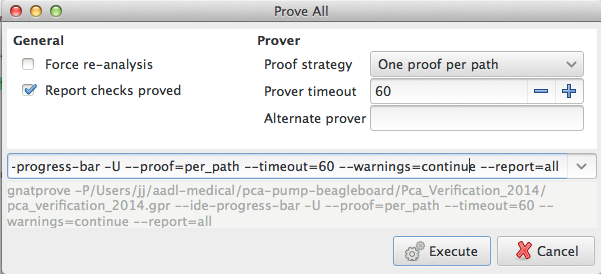
\includegraphics[width=0.7\textwidth]{figures/gnatprove-settings.png}        
    \end{center}
    \caption{GNATprove settings}
    \label{figure:gnatprove-settings}
\end{figure}

Summary of proof analysis is presented in listing \ref{listing:pca_pump_move_dosed_unit_spark2014_gnatprove}. Proof analysis returned three warnings: \lstinline{overflow check might fail} and one warning: \lstinline{contract case might fail}. It indicates the same problem like in verification with SPARK 2005 tools: overflow hazard. Additionally, there is a warning (\lstinline{postcondition might fail}) caused by tools limitations. If state refinement is not used (i.e. refined variables are defined in package specification), this warning does not occur. The same program without abstract state is presented in listing \ref{listing:pca_pump_move_dosed_unit_spark2014_no_refinement}. Its verification summary is shown in listing \ref{listing:pca_pump_move_dosed_unit_spark2014_gnatprove_no_refinement}. 

%http://docs.adacore.com/spark2014-docs/html/ug/spark_2014.html#abstract-state-refined-state-and-initializes

\singlespacing
\begin{lstlisting}[frame=single, gobble=0, caption={GNATprove verification summary of module for dose monitoring in SPARK 2014}, label={listing:pca_pump_move_dosed_unit_spark2014_gnatprove}]
analyzing Pca_Pump, 1 checks
analyzing Pca_Pump.Dosed_State, 0 checks
analyzing Pca_Pump.Dose_Volume_State, 0 checks
analyzing Pca_Pump.Sum, 3 checks
analyzing Pca_Pump.Read_Dosed, 4 checks
analyzing Pca_Pump.Increase_Dosed, 3 checks
analyzing Pca_Pump.Move_Dosed, 12 checks
pca_pump.adb:5:39: info: length check proved
pca_pump.adb:27:10: info: loop invariant initialization proved
pca_pump.adb:27:10: info: loop invariant preservation proved
pca_pump.adb:28:27: warning: overflow check might fail
pca_pump.adb:38:70: warning: overflow check might fail
pca_pump.adb:47:10: info: loop invariant initialization proved
pca_pump.adb:47:10: info: loop invariant preservation proved
pca_pump.adb:47:65: info: index check proved
pca_pump.adb:48:27: warning: overflow check might fail
pca_pump.adb:59:10: info: loop invariant initialization proved
pca_pump.adb:59:10: info: loop invariant preservation proved
pca_pump.adb:59:55: info: index check proved
pca_pump.ads:29:17: info: precondition proved
pca_pump.ads:29:48: info: overflow check proved
pca_pump.ads:36:14: warning: postcondition might fail, requires Dosed_State (Doses_Array_Index'Last) = 0
pca_pump.ads:37:6: info: disjoint contract cases proved
pca_pump.ads:37:6: info: complete contract cases proved
pca_pump.ads:37:66: warning: contract case might fail
pca_pump.ads:37:69: info: precondition proved
pca_pump.ads:37:86: info: precondition proved
pca_pump.ads:38:66: warning: contract case might fail
pca_pump.ads:38:69: info: precondition proved
pca_pump.ads:38:86: info: precondition proved
\end{lstlisting}
\doublespacing

\singlespacing
\begin{lstlisting}[language=ada2012, frame=single, gobble=0, caption={Sequential module for dose monitoring in SPARK 2014 without variable refinement}, label={listing:pca_pump_move_dosed_unit_spark2014_no_refinement}]
package Pca_Pump_No_Refinement
  with SPARK_Mode
is
   type Drug_Volume is range 0 .. 2**15-1;

   subtype Doses_Array_Index is Integer range 1 .. 60;
   type Doses_Array is array (Doses_Array_Index) of Drug_Volume;

   Dosed : Doses_Array := Doses_Array'(others => 0);
   Dose_Volume : Drug_Volume := 1;

   function Sum(Arr : Doses_Array) return Drug_Volume
     with Convention => Ghost;

   function Read_Dosed return Drug_Volume
     with Global  => (Input => (Dosed)),
     Pre     => Sum(Dosed) <= Drug_Volume'Last;

   procedure Increase_Dosed
     with Global  => (Input  => Dose_Volume, In_Out => Dosed),
     Depends => (Dosed => (Dosed, Dose_Volume)),
     Pre     => Read_Dosed <= Drug_Volume'Last - Dose_Volume;

   pragma Unevaluated_Use_Of_Old (Allow);

   procedure Move_Dosed
     with Global  => (In_Out => Dosed),
     Depends => (Dosed => Dosed),
     Post => (Dosed(Doses_Array_Index'Last) = 0),
     Contract_Cases => (Dosed(Doses_Array_Index'First) = 0 => Read_Dosed'Old = Read_Dosed,
                        Dosed(Doses_Array_Index'First) > 0 => Read_Dosed'Old > Read_Dosed);
end Pca_Pump_No_Refinement;

package body Pca_Pump_No_Refinement
  with SPARK_Mode
is
   function Sum(Arr : Doses_Array) return Drug_Volume
   is
      Result : Drug_Volume := 0;
   begin
      for I in Doses_Array_Index loop
         pragma Loop_Invariant (true);
         Result := Result + Arr(I);
      end loop;
      return Result;
   end Sum;

   procedure Increase_Dosed
   is
   begin
      Dosed(Doses_Array_Index'Last) := Dosed(Doses_Array_Index'Last) + Dose_Volume;
   end Increase_Dosed;

   function Read_Dosed return Drug_Volume
   is
      Result : Drug_Volume := 0;
   begin
      for I in Doses_Array_Index loop
         pragma Loop_Invariant (if I > 1 then Result >= Dosed (I-1));
         Result := Result + Dosed(I);
      end loop;
      return Result;
   end Read_Dosed;

   procedure Move_Dosed
   is
   begin
      for I in Doses_Array_Index range 1 .. Doses_Array_Index'Last-1 loop
         pragma Loop_Invariant (if I > 1 then Dosed (I-1) = Dosed (I));
         Dosed(I) := Dosed(I+1);
      end loop;
      Dosed(Doses_Array_Index'Last) := 0;
   end Move_Dosed;
end Pca_Pump_No_Refinement;
\end{lstlisting}
\doublespacing

\singlespacing
\begin{lstlisting}[frame=single, gobble=0, caption={GNATprove verification summary of module for dose monitoring in SPARK 2014 without variable refinement}, label={listing:pca_pump_move_dosed_unit_spark2014_gnatprove_no_refinement}]
analyzing Pca_Pump_No_Refinement, 1 checks
analyzing Pca_Pump_No_Refinement.Sum, 3 checks
analyzing Pca_Pump_No_Refinement.Read_Dosed, 4 checks
analyzing Pca_Pump_No_Refinement.Increase_Dosed, 3 checks
analyzing Pca_Pump_No_Refinement.Move_Dosed, 12 checks
pca_pump_no_refinement.adb:9:10: info: loop invariant initialization proved
pca_pump_no_refinement.adb:9:10: info: loop invariant preservation proved
pca_pump_no_refinement.adb:10:27: warning: overflow check might fail
pca_pump_no_refinement.adb:18:70: warning: overflow check might fail
pca_pump_no_refinement.adb:26:10: info: loop invariant initialization proved
pca_pump_no_refinement.adb:26:10: info: loop invariant preservation proved
pca_pump_no_refinement.adb:26:65: info: index check proved
pca_pump_no_refinement.adb:27:27: warning: overflow check might fail
pca_pump_no_refinement.adb:36:10: info: loop invariant initialization proved
pca_pump_no_refinement.adb:36:10: info: loop invariant preservation proved
pca_pump_no_refinement.adb:36:55: info: index check proved
pca_pump_no_refinement.ads:9:39: info: length check proved
pca_pump_no_refinement.ads:22:17: info: precondition proved
pca_pump_no_refinement.ads:22:48: info: overflow check proved
pca_pump_no_refinement.ads:29:14: info: postcondition proved
pca_pump_no_refinement.ads:30:6: info: disjoint contract cases proved
pca_pump_no_refinement.ads:30:6: info: complete contract cases proved
pca_pump_no_refinement.ads:30:60: warning: contract case might fail
pca_pump_no_refinement.ads:30:63: info: precondition proved
pca_pump_no_refinement.ads:30:80: info: precondition proved
pca_pump_no_refinement.ads:31:60: warning: contract case might fail
pca_pump_no_refinement.ads:31:63: info: precondition proved
pca_pump_no_refinement.ads:31:80: info: precondition proved
\end{lstlisting}
\doublespacing
